\section{黑洞}

\subsection{Schwarzschild 黑洞}

广义相对论中黑洞有三种形成机制：
\begin{enumerate}[label=(\arabic*)]
    \item 原初黑洞：早期宇宙密度涨落形成的原初小黑洞。
    \item 恒星级黑洞：大质量恒星演化的一种结局。
    \item 超大质量黑洞：星团或者星系核引力坍缩后形成的巨型黑洞。
\end{enumerate}

\subsubsection{Schwarzschild 坐标系}
\paragraph{Schwarzschild的奇点}
在 Schwarzschild 坐标系中，Schwarzschild 时空的度规写作：
\begin{align}
\mathrm{d}s^{2}
&=
- \left(1 - \frac{r_{\mathrm{s}}}{r}\right)\mathrm{d}t^{2}
+ \left(1 - \frac{r_{\mathrm{s}}}{r}\right)^{-1}\mathrm{d}r^{2}
+ r^{2}\,\mathrm{d}\Omega^{2}.
\label{eq:schwarzschild-metric-rs}
\end{align}
这个度规表示一个永久黑洞（虽然并不存在）外的真空引力场，其中 Schwarzschild 半径为：
\begin{align}
r_{\mathrm{s}} \equiv 2GM.
\label{eq:rs-def}
\end{align}
这个度规有两个奇异的点，$0$ 和 $r=r_{\mathrm{s}}$。$r=0$ 是一个真正的时空奇异点，而 $r=r_{\mathrm{s}}$ 只是坐标奇异点，源于 Schwarzschild 坐标系无法覆盖整个永久黑洞时空流形。
这一点类似于球坐标，球坐标南极和北极的方位角就是奇异的。判断一个点是不是真正的物理奇点可以通过计算坐标无关的物理量得到，比如Ricci标量，Schwarzschild时空的Ricci标量为：
\begin{align}
    R = 48GMr^{-6}
\end{align}
显然只有$r=0$一个奇点
通过检验一个在 Schwarzschild 时空中运动的粒子， 也可以验证$r_{\mathrm{s}}$ 处不是物理奇异的。
\begin{derivationnote}[Schwarzschild 半径不是物理奇异点]
    球对称情况下，只考虑径向，在 Schwarzschild 时空中运动粒子的运动方程是：
    \begin{align}
        \left(\frac{\mathrm{d}r}{\mathrm{d}\tau}\right)^{2}
        &= E^{2} - \left(1 - \frac{r_{\mathrm{s}}}{r}\right), \\
        \frac{\mathrm{d}t}{\mathrm{d}\tau}
        &= \frac{E}{1 - \frac{r_{\mathrm{s}}}{r}} .
    \end{align}
    那么对于处于无穷远处的观察者，在 $r\rightarrow r_{\mathrm{s}}$ 时，有：
    \begin{align}
        \frac{\mathrm{d}t}{\mathrm{d}\tau} &\rightarrow \infty, \\[4pt]
        \Rightarrow\quad
        \frac{\mathrm{d}r}{\mathrm{d}t}
        = \frac{\mathrm{d}r/\mathrm{d}\tau}{\mathrm{d}t/\mathrm{d}\tau}
        &\rightarrow 0 .
    \end{align}
    这说明对于无穷远处的观察者而言，粒子在接近 Schwarzschild 半径的时候，其速度会越来越慢直到“冻结”在 Schwarzschild 半径处。然而，如果我们取粒子本身的固有时，会发现 $\frac{\mathrm{d}r}{\mathrm{d}\tau}$ 并不趋于 $0$，而是有限值，所以在粒子本身看来，它可以毫无障碍地穿过 Schwarzschild 半径。取 $E^{2} = 1$ 的简单情况计算粒子从 $r = r_{0} \geq r_{\mathrm{s}}$ 到 $r = 0$ 处所花的时间，对于粒子掉落情况有：
    \begin{align}
        \frac{\mathrm{d}r}{\mathrm{d}\tau}
        = -\sqrt{\frac{r_{\mathrm{s}}}{r}}
        \quad\Rightarrow\quad
        \Delta \tau
        = r_{\mathrm{s}}^{-1/2}\,\frac{2}{3}\,r_{0}^{3/2} .
    \end{align}
    这就是说对粒子本身而言，穿过 Schwarzschild 半径并不会遇见任何阻碍，这个奇点不是物理的。
\end{derivationnote}

\paragraph{Schwarzschild的因果结构}
考虑在 Schwarzschild 时空中径向运动的光子，可以画出时空中的光锥线，进而讨论时空中的因果结构。由 \ref{eq:schwarzschild-metric-rs} 取类光条件 $\mathrm{d}s^{2}=0$ 得
\begin{align}
0
&=
- \left(1 - \frac{r_{\mathrm{s}}}{r}\right)\mathrm{d}t^{2}
+ \left(1 - \frac{r_{\mathrm{s}}}{r}\right)^{-1}\mathrm{d}r^{2},
\\[4pt]
\Rightarrow\quad
\frac{\mathrm{d}r}{\mathrm{d}t}
&=
\pm\left(1 - \frac{r_{\mathrm{s}}}{r}\right),
\label{eq:radial-null-dr-dt}
\end{align}
两个方程正负分别对应粒子掉落黑洞和离开黑洞。由 \ref{eq:radial-null-dr-dt} 得到
\begin{align}
\frac{\mathrm{d}t}{\mathrm{d}r}
&=
\pm\left(1 - \frac{r_{\mathrm{s}}}{r}\right)^{-1}
=
\pm\,\frac{r}{r-r_{\mathrm{s}}},
\end{align}
积分可得
\begin{align}
t
&=
\pm\left(r + r_{\mathrm{s}}\ln\left|\frac{r}{r_{\mathrm{s}}}-1\right|\right)
+ \text{const}.
\label{eq:radial-null-integrated}
\end{align}
取 $+$ 时，$r$ 随着 $t$ 增大而增大，表示光子向外逃逸；取 $-$ 时，$r$ 随着 $t$ 增大而减小，表示光子掉入黑洞。

为了描述的方便可以引入乌龟坐标（tortoise coordinate）$r_{*}$，定义为
\begin{align}
r_{*}
\equiv
r + r_{\mathrm{s}}\ln\left|\frac{r}{r_{\mathrm{s}}}-1\right|.
\label{eq:tortoise-def}
\end{align}
由此可得
\begin{align}
\mathrm{d}t
&=
\pm\,\mathrm{d}r_{*}
\quad\Rightarrow\quad
t \mp r_{*}
=
\text{const}.
\label{eq:null-lines-tortoise}
\end{align}
这就是说对一条特定的光线而言，$t \mp r_{*}$ 是一个常数，这个常数可以标定一个光线族。不妨取
\begin{align}
u
\equiv
t - r_{*},
\qquad
v
\equiv
t + r_{*},
\label{eq:null-coords-def}
\end{align}
这样 $u$、$v$ 分别对应向外、向内的光线。

\begin{derivationnote}[视界内外 $t$ 与 $r$ 的类时/类空角色交换]
Schwarzschild 度规在 $r\neq 0$ 的区域满足同一真空 Einstein 方程，但在视界 $r=r_{\mathrm{s}}$ 的内外，其坐标的因果意义发生交换。

当 $r>r_{\mathrm{s}}$ 时，$1-\frac{r_{\mathrm{s}}}{r}>0$，径向 $(t,r)$ 部分为
\begin{align}
\mathrm{d}s^{2}_{(t,r)}
=
- \left(1-\frac{r_{\mathrm{s}}}{r}\right)\mathrm{d}t^{2}
+ \left(1-\frac{r_{\mathrm{s}}}{r}\right)^{-1}\mathrm{d}r^{2},
\end{align}
从而
\begin{align}
g_{tt}=-\left(1-\frac{r_{\mathrm{s}}}{r}\right)<0,
\qquad
g_{rr}=\left(1-\frac{r_{\mathrm{s}}}{r}\right)^{-1}>0,
\end{align}
即 $t$ 为类时方向、$r$ 为类空方向。

当 $0<r<r_{\mathrm{s}}$ 时，$1-\frac{r_{\mathrm{s}}}{r}<0$，同一表达式可改写为
\begin{align}
\mathrm{d}s^{2}_{(t,r)}
=
\left(\frac{r_{\mathrm{s}}}{r}-1\right)\mathrm{d}t^{2}
-
\left(\frac{r_{\mathrm{s}}}{r}-1\right)^{-1}\mathrm{d}r^{2},
\end{align}
从而
\begin{align}
g_{tt}=\left(\frac{r_{\mathrm{s}}}{r}-1\right)>0,
\qquad
g_{rr}=-\left(\frac{r_{\mathrm{s}}}{r}-1\right)^{-1}<0,
\end{align}
时间方向应该是度规符号小于0的方向， 所以，$t$ 变为类空方向、$r$ 变为类时方向。
\end{derivationnote}



\subsubsection{Eddington 坐标系}

前文已经论述 Schwarzschild 坐标在 Schwarzschild 半径处的奇异性源自于坐标的选择，现在寻找可以消除这一奇异性的坐标。

\paragraph{Minkowski 渐进的 Eddington 坐标}
在面积半径从内到外取进Schwarzschild半径时，坐标时间发散是因为$r_s\ln{|\frac{r}{r_s}-1}|$的发散。这提示我们取坐标变换
\begin{align}
    \widetilde{r} &= r, \\
    \widetilde{t} &= t + r_{\mathrm{s}} \ln\left|\frac{r}{r_{\mathrm{s}}} - 1\right|.
\end{align}
在该坐标系下，时空线元为（不区分 $\mathrm{d}r$ 和 $\mathrm{d}\widetilde{r}$）：
\begin{align}
    \mathrm{d}s^{2}
    = -\left(1 - \frac{r_{\mathrm{s}}}{r}\right)\mathrm{d}\widetilde{t}^{2}
    + \frac{2r_{\mathrm{s}}}{r}\,\mathrm{d}r\,\mathrm{d}\widetilde{t}
    + \left(1+\frac{r_{\mathrm{s}}}{r}\right)\mathrm{d}r^{2}
    + r^{2}\,\mathrm{d}\Omega^{2}.
\end{align}
在类光条件 $\mathrm{d}s^{2} = 0$ 的条件下，解关于 $\frac{\mathrm{d}r}{\mathrm{d}\widetilde{t}}$ 的一元二次方程可以得到：
\begin{align}
    \frac{\mathrm{d}r}{\mathrm{d}\widetilde{t}} &= -1, \qquad \text{内行解},\\
    \frac{\mathrm{d}r}{\mathrm{d}\widetilde{t}} &= \frac{1 - \frac{r_{\mathrm{s}}}{r}}{1+\frac{r_{\mathrm{s}}}{r}}, \qquad \text{外行解}.
\end{align}
考察 $r$ 随 $\widetilde{t}$ 的变化关系就可以知道解的分类由来，积分可得所有的光锥线：
\begin{align}
    \widetilde{t} + r &= V, \\
    \widetilde{t} - r - 2r_{\mathrm{s}}\ln\left|\frac{r}{r_{\mathrm{s}}} -1\right| &= U.
\end{align}
对这个坐标系，粒子内行进入视界是毫无疑问可在有限时间穿过的，但是粒子外行穿过视界，会被“冻结”在视界上，也就是说它无法描述白洞的行为，由此被称为 \textbf{内行 Eddington 坐标}。

类似的可以引入 \textbf{外行 Eddington 坐标}：
\begin{align}
    \widetilde{t} &= t - r_{\mathrm{s}} \ln\left|\frac{r}{r_{\mathrm{s}}} - 1\right|, \\
    \widetilde{r} &= r .
\end{align}
通过类似的讨论可以发现，这个坐标只能描述粒子外行通过视界的行为，而内行进入视界会被“冻结”。这两个坐标分别描述了“黑洞”和“白洞”的行为。

\paragraph{非 Minkowski 渐进的 Eddington 坐标}
若进一步放弃“在 $r\rightarrow\infty$ 时度规显式回到闵氏形式”的要求，可以得到一个更加常用的形式，
\begin{align}
    \widetilde{t} &= t + r_{*}, \\
    \widetilde{r} &= r .
\end{align}
对应的微分变换是：
\begin{align}
    \mathrm{d}t
    = \mathrm{d}\widetilde{t}
    - \frac{\mathrm{d}r}{1 - \frac{r_{\mathrm{s}}}{r}} .
\end{align}
此时内行和外行光锥线为：
\begin{align}
    \widetilde{t} &= V, \\
    \widetilde{t} - 2r_{*} &= U.
\end{align}
同样地，这个坐标无法描述外行行为，称为 \textbf{内行 Eddington 坐标}，与之类似的可以定义 \textbf{外行 Eddington 坐标}：
\begin{align}
    \widetilde{t} = t - r_{*}.
\end{align}
Eddington 坐标在一定程度上解决了坐标奇点的问题，外行和内行 Eddington 坐标可以分别描述向内和向外穿过视界的行为，但是无法同时描述两种行为。

\subsubsection{Kruskal 坐标}
虽然 Eddington 坐标已经能描述黑洞或白洞的一方，但要同时覆盖黑洞与白洞区域，消除坐标奇异性就需要引入 Kruskal 坐标。
在$\ref{eq:null-coords-def}$中我们得到了两个标定光线族的数，不难发现 Eddington 其实就是使坐标时间t变换为$u$或者$v$，所以我们可以同时取$u$和$v$为坐标。
注意到在这种表示下，
\begin{align}
    ds^2 = -\left(1-\frac{r_s}{r}\right)du dv +r^2d\Omega^2
\end{align}
世界处仍然奇异，指数化得到：
\begin{align}
\widetilde{U}
&\equiv
\exp\left(-\frac{u}{2r_{\mathrm{s}}}\right) =\left(\frac{r}{r_s}-1\right)^{1/2}e^{\frac{r-t}{2r_s}}\Rightarrow \mathrm{d}u = -2r_{\mathrm{s}}\frac{\mathrm{d}\widetilde{U}}{\widetilde{U}}
\\
\widetilde{V}
&\equiv
\exp\left(\frac{v}{2r_{\mathrm{s}}}\right) =\left(\frac{r}{r_s}-1\right)^{1/2}e^{\frac{r+t}{2r_s}}\Rightarrow \mathrm{d}v =
2r_{\mathrm{s}}\frac{\mathrm{d}\widetilde{V}}{\widetilde{V}}
\label{eq:kruskal-UV-def}
\end{align}

由此度规可以写作：
\begin{align}
    \mathrm{d}s^{2}
    = \frac{4r_{\mathrm{s}}^{3}}{r}\exp\!\left(-\frac{r}{r_{\mathrm{s}}}\right)
      \mathrm{d}\widetilde{U}\,\mathrm{d}\widetilde{V}
      + r^{2}\,\mathrm{d}\Omega^{2}.
\end{align}
在这个坐标系中视界不存在奇异性。此时 Schwarzschild 坐标时间 $t$ 和面积半径 $r$ 都以隐函数的形式被决定：

对 $\widetilde{U}$ 和 $\widetilde{V}$ 进行线性组合可以得到另一种形式的 Kruskal 坐标：
\begin{align}
    X &= \frac{1}{2}\bigl(\widetilde{V} + \widetilde{U}\bigr) = \left(\frac{r}{r_s}-1\right)^{1/2}e^{\frac{r}{2r_s}}\cosh{\frac{t}{2r_s}},\\
    T &= \frac{1}{2}\bigl(\widetilde{V} - \widetilde{U}\bigr) = \left(\frac{r}{r_s}-1\right)^{1/2}e^{\frac{r}{2r_s}}\sinh{\frac{t}{2r_s}},
    \label{eq:XTandrs}
\end{align}
此时度规可写为
\begin{align}
    \mathrm{d}s^{2}
    = \frac{4 r_{\mathrm{s}}^{3}}{r}\exp\!\left(-\frac{r}{r_{\mathrm{s}}}\right)
      \bigl(-\mathrm{d}T^{2}+\mathrm{d}X^{2}\bigr)
      + r^{2}\,\mathrm{d}\Omega^{2}.
\end{align}

\subsection{其他的黑洞}
\subsubsection{Reissner--Nordstr\"om 黑洞}

在爱因斯坦--麦克斯韦理论中，电真空（仅含电磁场、无物质源）满足
\begin{align}
T_{\mu\nu}
&=
\frac{1}{\mu_{0}}
\left(
F_{\mu}{}^{\rho}F_{\nu\rho}
-\frac{1}{4}g_{\mu\nu}F^{\rho\sigma}F_{\rho\sigma}
\right),
\qquad
\nabla_{\mu}F^{\mu\nu}=0 .
\end{align}

将电磁场能动张量带入Einstein场方程，在球对称情况下，可以得到静态球对称带电黑洞解为 Reissner--Nordstr\"om（RN）度规和对应的四维电势（取 $G=1$）：
\begin{align}
\mathrm{d}s^{2}
&=
-\left(1-\frac{2M}{r}+\frac{Q^{2}}{r^{2}}\right)\mathrm{d}t^{2}
+\frac{\mathrm{d}r^{2}}{-g_{tt}}
+r^{2}\mathrm{d}\Omega^{2} \\
A_{\mu}&=\left(-\frac{Q}{r},\,0,\,0,\,0\right).
\end{align}

首先讨论其视界， $g_{tt}=0$ 时度规发散可得
\begin{align}
r^{2}-2Mr+Q^{2}=0
\quad\Rightarrow\quad
r_{\pm}=M\pm\sqrt{M^{2}-Q^{2}} .
\end{align}
可以发现：
\begin{enumerate}[label=(\arabic*)]
    \item $Q = 0$时，退化为Schwarzschild黑洞形式。
    \item $0 < \abs{Q} < M$时，有两个奇点$r_\pm$。
    \item $\abs{Q} = 0$时，$r_{\pm} = M$内外视界重合，这也被称为极端RN黑洞。
    \item $\abs{Q}>M$，关于视界的方程没有实根，不存在视界。这时，唯一存在一个物理上的奇点，并且这个奇点裸露在外没有视界的包围，称为裸奇点。
\end{enumerate}
Roger Penrose提出宇宙监督猜想，认为这种裸奇点并不存在。简单来说，如果裸奇点存在，物理世界中的光锥会延伸到物理奇点并终止于此，因果也在此被截断。
\paragraph{检验粒子测地线与有效势}
RN 时空中的不带电检验粒子仍然满足测地线，类似于 Schwarzschild 情形的讨论可知仍然有守恒量 $p_{t}$ 和 $p_{3}$，且总可选取 $\theta=\pi/2$（平面运动）。特别地，对于有质量粒子，径向方程为
\begin{align}
\left(\frac{\mathrm{d}r}{\mathrm{d}\tau}\right)^{2}
=
E^{2}
-\left(1-\frac{2M}{r}+\frac{Q^{2}}{r^{2}}\right)\left(1+\frac{L^{2}}{r^{2}}\right).
\end{align}
显然由于 $Q$ 的出现改变了 $r\to 0$ 时有效势的行为，使得 RN 黑洞的中心奇点有无穷高的势垒，不可能被检验粒子达到（除非是无质量且直接无角动量直接打向中心的粒子）。一般认为，RN 黑洞内视界之内的时空结构可能是不稳定的。

\subsubsection{Kerr 黑洞}

在真空爱因斯坦方程中，Kerr 于上世纪60年代得到了一个稳态轴对称解，其线元在 Boyer-Lindquist 坐标下为：
\begin{align}
\mathrm{d}s^{2} &= -\frac{\Delta}{\rho^{2}}(\mathrm{d}t - a\sin^{2}\theta \, \mathrm{d}\varphi)^{2} + \frac{\sin^{2}\theta}{\rho^{2}}[(r^{2}+a^{2})\mathrm{d}\varphi - a\mathrm{d}t]^{2} + \frac{\rho^{2}}{\Delta}\mathrm{d}r^{2} + \rho^{2}\mathrm{d}\theta^{2}, \label{eq:kerr_metric} \\
\rho^{2} &= r^{2} + a^{2}\cos^{2}\theta, \quad \Delta = r^{2} - 2Mr + a^{2}.
\end{align}
此度规描述了一个带角动量 $J = aM$ 的旋转黑洞。当比角动量 $a=0$ 时，Kerr 度规退化为质量为 $M$ 的史瓦西度规。
此度规的奇异性有两个情况$\rho^2 = 0$和$\Delta = 0$，分别对应物理奇异性和坐标奇异性。首先讨论其视界，坐标奇异性出现在 $\Delta=0$ 处，该处定义了 Kerr 黑洞的视界位置：
\begin{align}
r^{2} - 2Mr + a^{2} = 0 \quad \Rightarrow \quad r_{\pm} = M \pm \sqrt{M^{2} - a^{2}} .
\end{align}
可以发现：
\begin{enumerate}[label=(\arabic*)]
    \item $a = 0$ 时，退化为 Schwarzschild 黑洞形式，$r_{+} = 2M$ 和 $r_{-}=0$。
    \item $0 < |a| < M$ 时，存在两个视界 $r_{+}$（外视界）和 $r_{-}$（内视界）。
    \item $M = |a|$ 时，$r_{+} = r_{-} = M$，内外视界重合，称为极端 Kerr 黑洞。
    \item $M < |a|$ 时，关于视界的方程无实根，不存在视界，只有一个裸奇点。
\end{enumerate}

Kerr 黑洞的物理奇异性出现在 $\rho^{2}=0$ 处，即：
\begin{align}
r=0,\quad \theta = \pi/2.
\label{eq:sr in BL}
\end{align}
为看清其内禀结构，可通过坐标变换：
\begin{align}
\left\{\begin{array}{c}
\tilde{t}=t-r+\displaystyle\int \frac{r^{2}+a^{2}}{\Delta} \mathrm{d}r \\
x=(r \cos \tilde{\varphi}-a \sin \tilde{\varphi}) \sin \theta \\
y=(r \sin \tilde{\varphi}+a \cos \tilde{\varphi}) \sin \theta \\
z=r \cos \theta, \quad \tilde{\varphi}:=\varphi+\displaystyle\int \frac{a}{\Delta} \mathrm{d}r
\end{array}\right.
\end{align}
在此“直角坐标”下，奇异性表现为一个半径为 $a$ 的圆环：
\begin{align}
x^{2}+y^{2}=a^{2},\quad z=0,
\end{align}
故称为 \textbf{奇环}，它类似于Schwarzschild的奇点但又有很大的不同。从$\ref{eq:sr in BL}$可以知道，这个“点”实际上是一个半径为0,极角为$\pi/2$的圆环，如果从$\theta \neq \pi/2$的方向靠近$r=0$,则不会产生奇异性。
从对称性的角度也可以理解这一点，Schwarzschild黑洞是球对称的，奇点也有球对称性；Kerr黑洞是轴对称的，奇点就被角动量“展开”成一个具有轴对称性的环状结构。

本征频率和无穷远观察者观察到的频率有关系：$\sqrt{-g_{tt}} v_p = v_\infty$，令$\sqrt{-g_{tt}}= 0$可得其无限红移面（静界）：
\begin{align}
    r_{\pm}^s = M \pm \sqrt{M^2 - a^2\cos^2{\theta}} 
\end{align}
除两极 ($\theta=0,\pi$) 外，静界与外视界 $r_{+}$ 并不重合。Boyer-Lindquist坐标是渐进Minkovski的，且可以通过Killing方程证明$\partial_t$是一个Killing矢量。
Kerr黑洞的时空被其视界与无限红移面静界自然地划分为几个性质迥异的区域，其结构如下图所示（以赤道面切片示意）：
\begin{enumerate}
    \item \textbf{正常区（$r > r_+^s$）}：位于外无限红移面之外，观测者可以在此区域相对于无穷远保持静止，其物理行为与在弱场环境中类似。

    \item \textbf{（外）拖拽能层（$r_+ < r < r_+^s$）}：此时$g_{00}>0$，$\partial_t$成为类空的Killing矢量。如果粒子在这个区域内保持与无穷远观测者的静止，则会导致超光速。所以，在拖拽能层的粒子一定会受到Kerr黑洞的拖拽，随时空流动而不能保持相对于无穷远观测者的静止。

    \item \textbf{（外）单向膜区（$r_- < r < r_+$）}：此时度规径向分量为负，光锥朝向r的方向，为保证因果性，进入到此区域的粒子朝着r单向演化的方向运动，朝内的粒子一去不返。
    
    \item \textbf{内能层与内区（$r < r_-$）}：位于内视界之内,存在一个\textbf{内无限红移面}（$r_-^s$），它与内视界之间构成“内能层”。
    
    \item \textbf{奇环（$r = 0$且$\theta = \pi/2$）}
\end{enumerate}

\subsubsection{Kerr-Newman 黑洞}

\paragraph{度规与电磁势}
Kerr-Newman 黑洞是爱因斯坦-麦克斯韦理论（电真空爱因斯坦方程）中最一般的稳态轴对称解，在 Boyer-Lindquist 坐标下的线元与电磁四维势为：
\begin{align}
\mathrm{d}s^{2} &= -\frac{\Delta}{\rho^{2}}(\mathrm{d}t - a\sin^{2}\theta \, \mathrm{d}\varphi)^{2} 
+ \frac{\sin^{2}\theta}{\rho^{2}}\bigl[(r^{2}+a^{2})\mathrm{d}\varphi - a\mathrm{d}t\bigr]^{2} 
+ \frac{\rho^{2}}{\Delta}\mathrm{d}r^{2} + \rho^{2}\mathrm{d}\theta^{2} \label{eq:kn_metric1} \\
&= -\Bigl(1-\frac{2Mr-Q^{2}}{\rho^{2}}\Bigr) \mathrm{d}t^{2}
- 2\frac{(2Mr-Q^{2})a\sin^{2}\theta}{\rho^{2}} \mathrm{d}t\mathrm{d}\varphi \notag \\
&\quad + \Bigl(r^{2}+a^{2}+\frac{(2Mr-Q^{2})a^{2}\sin^{2}\theta}{\rho^{2}}\Bigr) \sin^{2}\theta \, \mathrm{d}\varphi^{2}
+ \frac{\rho^{2}}{\Delta}\mathrm{d}r^{2} + \rho^{2}\mathrm{d}\theta^{2}, \label{eq:kn_metric2} \\
A_{\mu} &= \Bigl(-\frac{Qr}{\rho^{2}},\; 0,\; 0,\; \frac{Qr a\sin^{2}\theta}{\rho^{2}}\Bigr), \label{eq:kn_potential}
\end{align}
其中
\begin{align}
\Delta &= r^{2} - 2Mr + a^{2} + Q^{2}, \quad 
\rho^{2} = r^{2} + a^{2}\cos^{2}\theta, \quad
a = \frac{J}{M}.
\end{align}
这里 $M$ 为黑洞质量，$Q$ 为电荷，$J$ 为角动量，$a$ 为单位质量的角动量。

\paragraph{视界与极端条件}
视界由 $\Delta=0$ 给出：
\begin{align}
r_{\pm} = M \pm \sqrt{M^{2} - a^{2} - Q^{2}}
        = \frac{GM}{c^{2}} \pm \sqrt{\Bigl(\frac{GM}{c^{2}}\Bigr)^{2} 
        - \Bigl(\frac{J}{Mc}\Bigr)^{2} - \frac{GQ^{2}}{c^{4}} } .
\end{align}
式中 $r_{+}$ 为外视界，$r_{-}$ 为内视界。黑洞参数需满足 $M^{2} \geq a^{2} + Q^{2}$ 以保证视界存在。当 $M^{2} = a^{2} + Q^{2}$ 时，内外视界重合，称为极端 Kerr-Newman 黑洞；若 $M^{2} < a^{2} + Q^{2}$，则不存在视界，出现裸奇点，违背宇宙监督假设。

\paragraph{黑洞无毛定理与热力学类比}
Kerr-Newman 解描述了一个带电荷 $Q$ 与角动量 $J$ 的旋转黑洞（简称 KN 黑洞），其时空结构与 Kerr 黑洞相似，但多了电荷的贡献。根据黑洞无毛定理，稳态黑洞仅由质量 $M$、电荷 $Q$ 和角动量 $J$ 三个宏观参数完全决定，其他任何细节信息（“毛发”）在引力坍缩过程中都会丢失。这一性质与热力学系统达到平衡态时仅由少数宏观参量描述相似。进一步，黑洞的演化趋向于稳态的过程，与非平衡系统趋向热平衡的过程在形式上高度相似，这为黑洞热力学的建立提供了基础。

\subsection{时空的几何结构与彭罗斯图}
\subsubsection{Kruskal图}
根据Kruskal坐标与Schwarzschild坐标之间的隐函数关系$\ref{eq:XTandrs}$，可以得到：
\begin{align}
    X^2 - T^2 &= \widetilde{U} \widetilde{V} = \left(\frac{r}{r_2}-1\right)\exp(\frac{r}{r_s}) \\
    \frac{X}{T} &= \tanh(\frac{t}{2r_s})
\end{align}
这就是说，在Kruskal坐标系中，“等时面”（时指Schwarzschild坐标系中的坐标时间）是经过原点的直线而“等距面”是双曲线。
根据我们原来的定义，X和T都大于0,这里实际上给坐标作了一个延拓。
\begin{figure}[H]
    \centering
    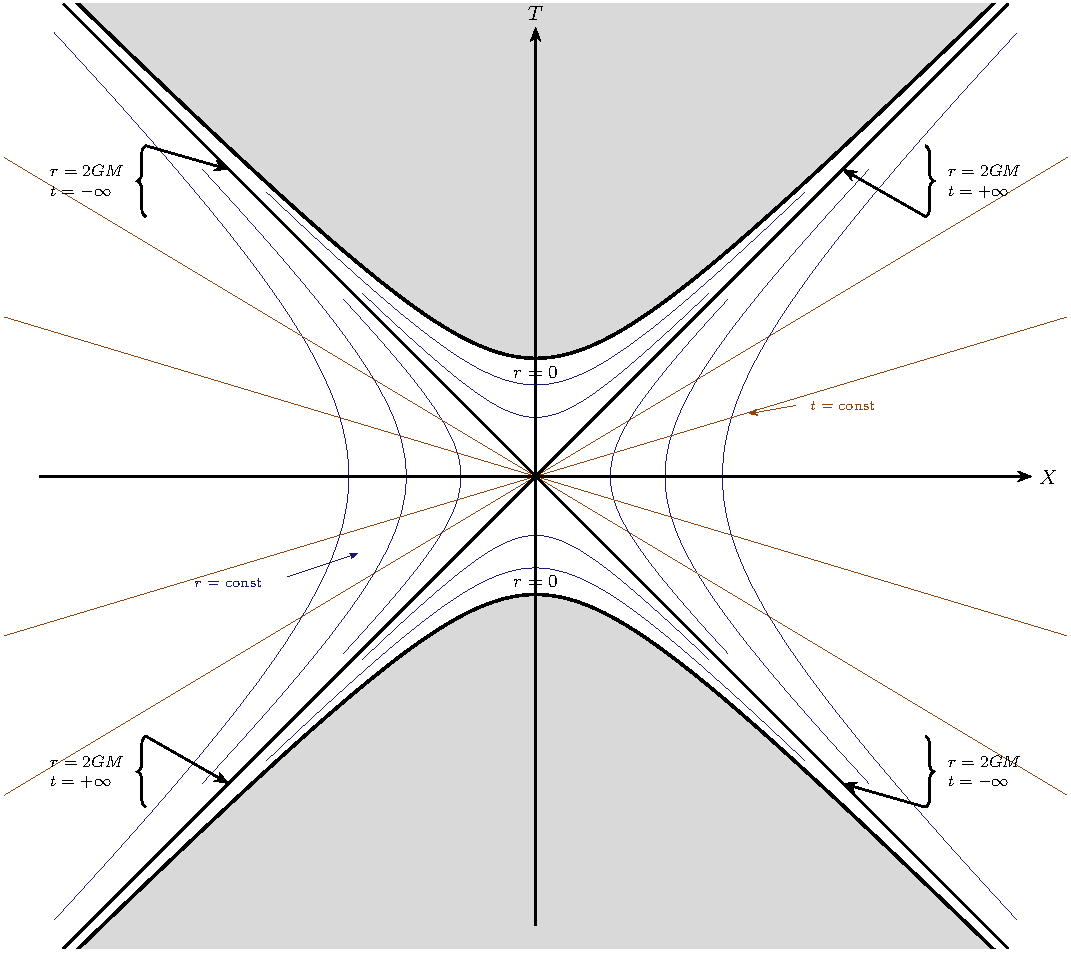
\includegraphics[width = .8\linewidth]{figs/Kruskal_Diagram.pdf}
    \caption{Kruskal图}
\end{figure}
可以看见，整个时空被kruskal坐标划分为四个区域：
\begin{enumerate}[label = \Roman*.]
    \item 外部宇宙：黑洞外部的宇宙，这就是我们所处的时空。
    \item 黑洞内部：此时类时坐标指向奇点，粒子朝着物理奇点前进。Schwarzschild坐标系中，视界内外类时分量变成r，也就是说为保持因果粒子会不可避免的向奇点演化。Kruskal坐标中这一点体现在光锥是$45\degree$开口的，在区域$\mathrm{II}$中未来光锥一定会包含奇点面。
    \item 白洞内部：这是一个与II完全相反的区域，黑洞的时间反演，也就是所谓的白洞。在这里，光锥的过去是奇点而未来是视界。
    \item 对称宇宙的外部：白洞的外部，和我们的宇宙对称。
\end{enumerate}

\subsubsection{Einstein-Rosen桥}
把坐标延拓到$\widetilde{U}$和$\widetilde{V}$小于0的区域，可以发现另一个宇宙。通过坐标时间$t=0$的切片，可以到处连接两个区域的Einstein-Rosen桥
\paragraph{空间几何的嵌入与各向同性坐标}
选取 Kruskal 时空的 $t=0$ 切片（对应 $U=V=0$ 的水平线）。在此切片上，原 Schwarzschild 空间度规（$r > 2GM$）为：
\begin{equation}
    ds^2 = \left(1 - \frac{2GM}{r}\right)^{-1} dr^2 + r^2 (d\theta^2 + \sin^2\theta d\phi^2) \label{eq:sch_spatial}
\end{equation}
为了描述跨越视界（$r=2GM$）的整体几何，引入新的径向坐标 $\rho$，定义如下变换：
\begin{equation}
    r = \rho \left(1 + \frac{GM}{2\rho}\right)^2 = \rho + GM + \frac{G^2M^2}{4\rho} \label{eq:iso_trans}
\end{equation}
该变换具有双值性：对于任意 $r > 2GM$，存在两个 $\rho$ 值（互为倒数关系 $\rho \leftrightarrow G^2M^2/4\rho$），视界 $r=2GM$ 对应于唯一不动点 $\rho = GM/2$。
利用恒等式 $\left(1-\frac{2GM}{r}\right) = \frac{(1-GM/2\rho)^2}{(1+GM/2\rho)^2}$ 并计算微分 $dr$可得度规：
\begin{equation}
    ds^2 = \left(1 + \frac{GM}{2\rho}\right)^4 \left[ d\rho^2 + \rho^2 (d\theta^2 + \sin^2\theta d\phi^2) \right]
\end{equation}
\begin{enumerate}
    \item \textbf{渐近行为：} 当 $\rho \to \infty$ 时，度规趋于平直欧几里得空间 $\mathbb{R}^3$；由于变换的对称性，当 $\rho \to 0$ 时，度规同样趋于平直 $\mathbb{R}^3$。这证实了时空连接着两个独立的渐近平直宇宙。
    \item \textbf{喉部结构（Throat）：} 在 $\rho = GM/2$ 处，$r$ 取得最小值 $2GM$。此处是一个极小曲面，称为\textbf{分叉球（Bifurcation Sphere）}。
    \item \textbf{爱因斯坦-罗森桥：} 这种几何结构即为连接两个宇宙的虫洞。但需注意，该虫洞不仅不可通过，且其路径是类空的。
\end{enumerate}

\subsubsection{嵌入图的时间演化：从连接到断裂（From Gemini）}

为了理解虫洞的动态断裂过程（即图 A-E 的演化），我们需要在 Kruskal 度规下计算 $T = \text{const} \neq 0$ 的空间切片形状。

\paragraph{1. 切片度规的导出}
从 Kruskal 全时空线元出发：
\begin{equation}
    ds^2 = \frac{32M^3}{r} e^{-r/2M} (-dT^2 + dX^2) + r^2 d\Omega^2
\end{equation}
其中 $r$ 由隐函数关系定义：
\begin{equation}
    X^2 - T^2 = \left(\frac{r}{2M} - 1\right) e^{r/2M} \label{eq:kruskal_implicit}
\end{equation}
选取某一时刻 $T = T_0$（常数），则 $dT=0$。考察赤道面 $\theta = \pi/2$，度规简化为：
\begin{equation}
    dl^2_{slice} = \frac{32M^3}{r} e^{-r/2M} dX^2 + r^2 d\phi^2
\end{equation}
为了画出以 $r$ 为参数的形状，需将 $dX$ 转换为 $dr$。对式 \eqref{eq:kruskal_implicit} 两边微分（保持 $T$ 不变）：
\begin{align}
    2X dX &= \frac{d}{dr}\left[ \left(\frac{r}{2M} - 1\right) e^{r/2M} \right] dr \\
    &= \frac{r}{4M^2} e^{r/2M} dr
\end{align}
从而得到变换关系：
\begin{equation}
    dX^2 = \frac{r^2 e^{r/M}}{64M^4 X^2} dr^2 = \frac{r^2 e^{r/M}}{64M^4 \left[ T^2 + (\frac{r}{2M}-1)e^{r/2M} \right]} dr^2
\end{equation}
将此代回切片度规，得到该时刻的纯空间线元：
\begin{equation}
    dl^2_{slice} = \left[ 1 + \frac{T^2}{T^2 + (\frac{r}{2M}-1)e^{r/2M}} \right] \left(1-\frac{2M}{r}\right)^{-1} dr^2 + r^2 d\phi^2
    \label{eq:dynamic_metric}
\end{equation}
(注：此处经过了一定的代数化简，利用了 $1/(1-2M/r) = r/(r-2M)$ 的关系)。

\paragraph{2. 嵌入方程与喉部动力学}
将上述二维弯曲面嵌入三维欧几里得空间（圆柱坐标 $z, r, \phi$），线元匹配条件为：
\begin{equation}
    dl^2_{Euclid} = \left[ 1 + \left(\frac{dz}{dr}\right)^2 \right] dr^2 + r^2 d\phi^2
\end{equation}
比较 $dr^2$ 的系数，可得嵌入曲面 $z(r)$ 的斜率方程：
\begin{equation}
    \left(\frac{dz}{dr}\right)^2 = \frac{2M}{r-2M} + \frac{T^2}{(1-\frac{2M}{r})\left[ T^2 + (\frac{r}{2M}-1)e^{r/2M} \right]}
\end{equation}
这个复杂的式子决定了不同 $T$ 时刻切片的具体形状。然而，决定虫洞是否连通的关键在于\textbf{喉部（Throat）}的存在性。

\begin{derivationnote}[喉部半径的演化]
    几何上，喉部对应于嵌入图的最窄处，即 $r$ 无法取到更小值的点。在 Kruskal 图中，这对应于左右宇宙的分界线 $X=0$。
    令 $X=0$，代入隐函数方程 \eqref{eq:kruskal_implicit}，我们得到喉部半径 $r_{min}$ 与时间 $T$ 的关系：
    \begin{equation}
        -T^2 = \left(\frac{r_{min}}{2M} - 1\right) e^{r_{min}/2M}
    \end{equation}
    定义函数 $f(r) = (r/2M - 1)e^{r/2M}$，其性质如下：
    \begin{itemize}
        \item 最小值：在 $r=0$ 处，$f(0) = -1$。
        \item 零点：在 $r=2M$ 处，$f(2M) = 0$。
    \end{itemize}
    据此分析图 A-E 的物理过程：
    \begin{enumerate}
        \item \textbf{图 C ($T=0$)}：方程为 $f(r_{min}) = 0$，解得 $r_{min} = 2M$。此时虫洞最宽，连接完好。
        \item \textbf{图 B, D ($0 < |T| < 1$)}：方程为 $f(r_{min}) = -T^2$（介于 $-1$ 和 $0$ 之间）。此时方程有唯一解 $0 < r_{min} < 2M$。说明虫洞依然连通，但喉部半径随着 $|T|$ 增大而迅速收缩。
        \item \textbf{图 A, E ($|T| \geq 1$)}：方程变为 $f(r_{min}) \leq -1$。由于 $f(r)$ 的最小值为 $-1$（对应 $r=0$），当 $|T| > 1$ 时方程\textbf{无解}。物理上意味着切片在延伸到中心之前就已终止于奇点 ($r=0$)，空间不再连通，虫洞断裂为两个分离的尖点。
    \end{enumerate}
\end{derivationnote}
\subsubsection{彭罗斯图}
类似于Riemann球，彭罗斯图把无穷处的时空映射到有限的地方，取：
\begin{align}
    \widetilde{U} = \tan{\frac{\pi}{2}x} \\
    \widetilde{V} = \tan{\frac{\pi}{2}y}
\end{align}
\subsubsection{Penrose 过程}

Kerr 黑洞存在一个特殊的区域——\textbf{能层}，Roger Penrose 提出理论上可以从旋转黑洞中提取能量。具体的实现过程称为\textbf{Penrose 过程}。
\n{默认使用Boyer-Lindquist坐标，这个坐标系中t相当于无穷远处的静止观测者经历的时间。}
Kerr时空中存在对应于时间平移不变性的 Killing 矢量场 $\xi^{\mu} = (1, 0, 0, 0)$。对于一个在测地线上运动的粒子，其四动量为 $p^{\mu}$，则无穷远处的观测者测得的守恒能量 $E$ 定义为：
\begin{align}
E = -p_{\mu}\xi^{\mu} = -g_{\mu\nu}p^{\mu}\xi^{\nu}.
\end{align}
\n{Boyer-Lindquist坐标中有沿着时间方向的Killing矢量，粒子的测地线沿着Killing矢量的分量在无穷远观测者看来就是能量。}
设想一个实验：从无穷远处的实验室向黑洞释放一个能量为 $E_0$ 的检验粒子（粒子0）。当粒子进入能层后，分裂为两个碎片，分别记为粒子1和粒子2。根据局域的四动量守恒 $p_0^{\mu} = p_1^{\mu} + p_2^{\mu}$，能量满足线性叠加关系：
设能量为$E_0$的检验粒子释放向黑洞运动，进入能层后分裂为粒子1和粒子2,由四动量守恒
\begin{align}
    p^{\mu}_0 = p^{\mu}_1 + p^{\mu}_2
\end{align}
等式对$\xi_{\mu}$缩并有，
\begin{align}
E_0 = E_1 + E_2.
\end{align}
\n{此时还没进入视界内，通过势垒散射或者粒子1的能量转移可以让粒子2获取足够的能量逃离能层回到静界。}

两个粒子其中一个粒子1掉落黑洞而粒子2逃离至无穷远，若 $E_1 < 0$，则逃逸回无穷远的粒子2的能量 $E_2 = E_0 - E_1$ 将大于初始能量 $E_0$，我们以损失粒子1为代价，将黑洞的能量转移到粒子2并提取出来。

\paragraph{“负能”的存在}
 虽然使用Boyer-Lindquist 全局坐标系，但标量的值不依赖于坐标系选择，我们可以在时空中的某一点选取最简便的坐标系来判断其正负。

\begin{enumerate}
    \item \textbf{在能层外（$g_{00} < 0$）：}
    Killing 矢量类时,由于 $E$ 是标量，我们选取一个随粒子运动的局域惯性系。在此参考系中，粒子静止，其四动量为 $\tilde{p}^{\mu} = (m, 0, 0, 0)$ ($m>0$)。
    则在此坐标系中$\tilde{\xi}^{2} = -\tilde{\xi}^2_{t}+\tilde{\xi}^2_{i} < 0$，$\tilde{\xi}^t>0$，能量为：
    \begin{align}
        E = -\eta_{\mu\nu}\tilde{p}^{\mu}\tilde{\xi}^{\nu} = -(-1) \cdot m \cdot \tilde{\xi}^0 = m \tilde{\xi}^0 > 0.
        \label{cond:xi}
    \end{align}
    \item \textbf{在能层内（$g_{00} > 0$）：}
    此时Killing 矢量类空，不是因果保持的方向。没有类似\eqref{cond:xi}的限制，能量不必大于0，负能情况粒子处于极深的引力势井内，引力势能绝对值大于粒子动能与静能之和。
\end{enumerate}
这意味着在能层存在着“负能区域”，可以使得粒子1落入黑洞视界（$E_1 < 0$），粒子2逃逸到无穷远，观测者获得净能量。

\paragraph{黑洞参数演化与效率极限}
彭罗斯过程并非永动机，检验粒子忽略了粒子对黑洞的影响。但实际上，能量的提取是以消耗黑洞的能量为代价的。负能粒子的掉落会削减黑洞的质量，并且它的角动量与黑洞相反，会减缓黑洞的旋转，逐步缩小能层。最终Kerr黑洞退化为Schwarzschild黑洞，无法继续Penrose过程，因此Schwarzschild也被称为“死去的黑洞”。
根据\textit{黑洞面积不减定理}，在经典过程中视界表面积 $A$ 不减。
考虑一个初始为极端 Kerr 黑洞（$J=M^2$, $a=M$）的状态，通过反复的彭罗斯过程将角动量全部提取殆尽，使其退化为 Schwarzschild 黑洞（$J=0$）
能量提取的最大效率 $\eta$ 为：
\begin{align}
\eta_{\text{max}} = \approx 29\%.
\end{align}
对于带电的Newmann黑洞，情况是类似的，Penrose过程使得黑洞带电量下降，视界面积上升，能层减小。

\subsubsection{Kerr 时空中的粒子运动与ISCO}
比起Schwarzschild时空，Kerr时空中时空交叉，所以更麻烦。但是，依然可以使用时空中的守恒量进行化简。
由于 Kerr 时空具有时间平移不变性（1,0,0,0）和空间旋转不变性(0,0,1,0)，粒子运动存在两个守恒量,对于质量为 $m$ 的粒子，其四动量分量可以写为：
\begin{align}
p_t &= m g_{tt} \frac{d t}{d \tau} + m g_{t\phi} \frac{d\phi}{d\tau} = -mE, \\
p_\phi &= m g_{\phi t} \dot{t} + m g_{\phi\phi} \dot{\phi} = mL.
\end{align}
这是一组关于 $\dot{t}$ 和 $\dot{\phi}$ 的线性方程组。解出 $\dot{t}$ 和 $\dot{\phi}$可以得到：
\begin{align}
\rho^2 \frac{dt}{d\tau} &= -a(aE\sin^2\theta - L) + (r^2+a^2)\frac{P}{\Delta}, \\
\rho^2 \frac{d\phi}{d\tau} &= -\left(aE - \frac{L}{\sin^2\theta}\right) + \frac{aP}{\Delta}.
\end{align}
其中$\rho^2 = r^2 + a^2\cos^2\theta$， $P(r) = E(r^2+a^2) - aL$，$\Delta = r^2 -2Mr +a^2 + Q^2$

将上述速度分量代入四速度的归一化条件 $g_{\mu\nu}\frac{dx^\mu}{d\tau}\frac{dx^\nu}{d\tau} = -1$，可以得到：
\begin{align}
\left( -1 - \frac{2Mr(r^2+a^2)}{\Delta \rho^2} \right) E^2 + \frac{4Mar}{\Delta \rho^2}EL + \frac{\rho^2 - 2Mr}{\Delta \rho^2 \sin^2\theta}L^2 + \frac{\rho^2}{\Delta}\left(\frac{dr}{d\tau}\right)^2 + \rho^2 \left(\frac{d\theta}{d\tau}\right)^2 = -1.
\end{align}
仅有的轴对称性让粒子不一定做平面运动，这也是Kerr时空比Schwarzschild时空更复杂的地方。但是，不难察觉$\theta = \pi/2$的特殊平面运动仍然存在。此外，这个体系还有一个额外的守恒量——\textbf{Carter常数}。
\n{类似氢原子几何上只有SO(3)对称性，但中心势场带来了一个额外的对称性以及以及对应的守恒量——Longe-Kuta矢量。}
\paragraph{赤道面上的径向方程 ($\theta = \pi/2$)}
此时 $\theta = \pi/2, \dot{\theta} = 0, \sin\theta = 1, \cos\theta = 0, \rho^2 = r^2$。
代入主方程：
\begin{align}
r^4 \left(\frac{dr}{d\tau}\right)^2 - 2Mr(r^2+a^2)E^2 + 4Mra EL + (\Delta - a^2)L^2 = \Delta r^2 (E^2 - 1).
\end{align}
进一步整理为关于 $\left(\frac{dr}{d\tau}\right)^2$ 的显式：
\n{这里的 $W(r)$ 类似经典力学中“有效动能”（常数 - 有效势能）}
\begin{align}
r^4 \left(\frac{dr}{d\tau}\right)^2 = r^2 \left[ (r^2+a^2)E^2 - L^2 - \Delta \right] + 2Mr(aE - L)^2 \\
\left(\frac{dr}{d\tau}\right)^2 = E^2 - 1 + \frac{2M}{r} + \frac{a^2 E^2 - L^2 - a^2}{r^2} + \frac{2M}{r^3}(aE - L)^2 := W(r).
\end{align}

\paragraph{最小稳定圆轨道 (ISCO)}
圆轨道的存在及其稳定性由 $W(r)$ 的性质决定：
\begin{itemize}
    \item \textbf{轨道存在条件}：$W = 0$（径向速度为零）。
    \item \textbf{圆轨道条件}：$W' = dW/dr = 0$（径向受力平衡，势能极值点）。
    \item \textbf{轨道稳定性}：$W'' < 0$ 对应不稳定平衡，$W'' > 0$ 对应稳定平衡。
\end{itemize}

ISCO是稳定与不稳定轨道的临界点，即势能的拐点：
\begin{align}
W(r) = 0, \quad W'(r) = 0, \quad W''(r) = 0.
\end{align}
联立这三个方程可以解出 ISCO 的半径 $r_{\text{ISCO}}$ 以及对应的能量 $E$ 和角动量 $L$。

\textbf{极端Kerr黑洞(比角动量a=M)}的最小稳定圆轨道能量$E \approx 58\%$,粒子进入该轨道会释放$42\%$的能量。Kerr 黑洞的吸积过程是宇宙中极高效率的能量转换机制，这解释了类星体和活动星系核（AGN）的高光度来源。
若粒子的角动量满足\textbf{$L = aE$}时，径向方程中的 $(aE-L)^2$ 项消失，方程极大简化：
\begin{align}
\left(\frac{dr}{d\tau}\right)^2 = E^2 - \left( 1 - \frac{2M}{r} + \frac{a^2}{r^2} \right).
\end{align}
\n{这一点不难想象，因为这种情况下粒子的角动量和黑洞角动量相同}
若粒子落入黑洞，黑洞的质量变化 $\delta M = E$，角动量变化 $\delta J = L$。
由于 $L = aE$，则有：
    \begin{align}
        \frac{\delta J}{\delta M} = \frac{L}{E} = a \quad \Rightarrow \quad \delta \left(\frac{J}{M}\right) = \delta a = 0.
    \end{align}
    这意味着吞噬此类粒子\textbf{不会改变黑洞的比角动量 $a$}。
    对于 $L=aE$ 的粒子，其有效势能项包含 $+a^2/r^2$（排斥势）。当 $r \to 0$ 时，势垒趋于无穷大。因此，除非 $E$ 无穷大，否则粒子无法到达 $r=0$ 处。这体现了 Kerr 奇环的不可到达性（对于此类测地线而言）。
\section{扩展}
\subsection{作用量原理与引力场方程}
考虑一个质量为 $m$ 的自由粒子在弯曲时空中的运动。其作用量 $I$ 正比于粒子世界线的固有长度（固有时 $\tau$）：
\begin{align}
I = -m \int d\tau = -m \int \sqrt{-g_{\mu\nu}(x) \frac{dx^\mu}{d\lambda} \frac{dx^\nu}{d\lambda}} \, d\lambda,
\end{align}
其中 $\lambda$ 为世界线的任意参数。
令 $\delta I = 0$，即得\textbf{测地线方程}：
\begin{align}
\frac{d^2x^\sigma}{d\tau^2} + \Gamma^\sigma_{\mu\nu} \frac{dx^\mu}{d\tau} \frac{dx^\nu}{d\tau} = 0,
\end{align}
\n{不难验证这个作用量具有世界线重参数化不变性和电磁规范不变性}
带电粒子在电磁场中的作用量为
\begin{align}
I = \int \left( -m\sqrt{-g_{\mu\nu}\dot{x}^\mu\dot{x}^\nu} + q A_\mu(x) \dot{x}^\mu \right) d\lambda.
\end{align}

\paragraph{Einstein-Hilbert作用量}
广义相对论中考虑弯曲时空，计算作用量需要考虑标量函数在时空流形上的积分：
\n{不过我们没有交代标量函数在时空流形上的积分为什么是这个形式，那会牵扯太多的微分几何知识。但是这个形式满足的积分测度是微分同胚不变的，因为坐标变换下：
\[det(g_{\mu \nu}) = |\frac{\partial \tilde{x}}{\partial x}|^2 \tilde{g} \]
\[d^4 x = |\frac{\partial x}{\partial \tilde{x}}| d^4  \tilde{x}\]积分测度在坐标变换下不变。}
\begin{align}
    \int f(x) \sqrt{-g}d^4x
\end{align}
Einstein-Hilbert作用量为：
\begin{align}
I_G = \int R \sqrt{-g} \, d^4x = \int g^{\mu\nu} R_{\mu\nu} \sqrt{-g} \, d^4x.
\end{align}
对其进行变分：
\begin{align}
\delta I_G = \int \left( \delta g^{\mu\nu} R_{\mu\nu} + g^{\mu\nu} \delta R_{\mu\nu} + R \frac{\delta \sqrt{-g}}{\sqrt{-g}} \right) \sqrt{-g} \, d^4x.
\end{align}
这里需要用到两个关键的恒等式：
\begin{enumerate}
    \item \textbf{行列式的变分}：
        \begin{align}
            \delta \sqrt{-g} = -\frac{1}{2}\sqrt{-g} g_{\mu\nu} \delta g^{\mu\nu}
        \end{align}
    \item \textbf{Palatini 恒等式}（Ricci 张量的变分）：
    \begin{align}
    \delta R_{\mu\nu} = \nabla_\rho (\delta \Gamma^\rho_{\mu\nu}) - \nabla_\nu (\delta \Gamma^\rho_{\mu\rho}).
    \end{align}
\end{enumerate}

\n{恒等式的证明，还需要再复习。}
将 Palatini 恒等式代入作用量变分的中间项：
\begin{align}
\int g^{\mu\nu} \delta R_{\mu\nu} \sqrt{-g} d^4x = \int \nabla_\rho (g^{\mu\nu} \delta \Gamma^\rho_{\mu\nu} - g^{\mu\rho} \delta \Gamma^\nu_{\mu\nu}) \sqrt{-g} d^4x.
\end{align}
根据高斯定理，该项是一个全散度项，可以转化为边界上的积分。在经典的变分问题中，如果固定边界上的度规及其一阶导数（或引入 Gibbons-Hawking-York 边界项抵消），此项为零。
于是，变分结果仅剩下：
\begin{align}
\delta I_G = \int \left( R_{\mu\nu} - \frac{1}{2} R g_{\mu\nu} \right) \delta g^{\mu\nu} \sqrt{-g} \, d^4x.
\end{align}
令 $\delta I_G = 0$，即得到真空场方程 $G_{\mu\nu} = R_{\mu\nu} - \frac{1}{2}Rg_{\mu\nu} = 0$。

\paragraph{物质场的耦合与能量动量张量}
当存在物质场时，总作用量为
\begin{align}
    I = \int \left(\frac{R}{16\pi G} + \mathcal{L}_{mat}\right)\sqrt{-g}d^4x
\end{align}
物质场的能量动量张量 $T^{\mu\nu}$ 是物质作用量对度规的变分导数：
\n{这个定义与场论中由诺特荷定义的能动张量不一样，二者在简单的平直时空中才相同。}
\begin{align}
T_{\mu\nu} \equiv \frac{-2}{\sqrt{-g}} \frac{\delta }{\delta g^{\mu\nu}} \int \mathcal{L} \sqrt{-g} d^4x
\end{align}
总作用量的变分原理 $\delta I = 0$ 给出完整的爱因斯坦场方程：
\begin{align}
G_{\mu\nu} = 8\pi G T_{\mu\nu}.
\end{align}

\paragraph{实标量场的耦合}
以质量为 $m$ 的自由实标量场 $\phi$ 为例，其拉格朗日量为：
\begin{align}
\mathcal{L}_{\text{mat}} = -\frac{1}{2} g^{\mu\nu} \nabla_\mu \phi \nabla_\nu \phi - \frac{1}{2} m^2 \phi^2.
\end{align}
利用上述定义计算 $T_{\mu\nu}$。注意到 $\frac{\delta g^{\alpha\beta}}{\delta g^{\mu\nu}} = \delta^\alpha_\mu \delta^\beta_\nu$，且 $\delta \sqrt{-g} = -\frac{1}{2}\sqrt{-g} g_{\mu\nu} \delta g^{\mu\nu}$。
\n{标量场协变导数作用等同于普通导数}
\begin{align}
\delta (\mathcal{L}\sqrt{-g}) &= \delta \mathcal{L} \sqrt{-g} + \mathcal{L} \delta \sqrt{-g} \notag \\
&= \left( -\frac{1}{2} \delta g^{\alpha\beta} \partial_\alpha \phi \partial_\beta \phi \right) \sqrt{-g} - \frac{1}{2} g_{\mu\nu} \delta g^{\mu\nu} \mathcal{L} \sqrt{-g} \notag \\
&= -\frac{1}{2} \sqrt{-g} \delta g^{\alpha\beta} \left( \partial_\alpha \phi \partial_\beta \phi + g_{\alpha\beta} \mathcal{L} \right).
\end{align}
代入 $T_{\mu\nu}$ 的定义式：
\begin{align}
T_{\mu\nu} = \nabla_\mu \phi \nabla_\nu \phi - \frac{1}{2} g_{\mu\nu} \left( (\nabla\phi)^2 + m^2\phi^2 \right).
\end{align}
对于闵氏时空（Flat Space）中的静态场，考察其能量密度 $T^{00}$：
\begin{align}
T^{00} = (\partial_t \phi)^2 + \frac{1}{2} \left[ -(\partial_t \phi)^2 + (\nabla \phi)^2 + m^2 \phi^2 \right] = \frac{1}{2} \left[ (\partial_t \phi)^2 + (\nabla \phi)^2 + m^2 \phi^2 \right] > 0.
\end{align}
这表明该标量场满足能量密度为正的物理条件（弱能量条件）。